\newpage

\begin{multicols}{2}
\setcounter{page}{2}
\begin{tabular}{|*{14}{c|}}
\hline
   Имя  & 1 & 2 & 3 & 4 & 5 & 6 & 7 & 10 & 11 & ... & 24\\
  \hline
  Петя & 1 & 0 & 0 & 0 & 1 & 0 & 0 & 0 & 1 & 0 & 0 & 0 & 0\\
  \hline
  Коля & 0 & 1 & 0 & 0 & 0 & 1 & 0 & 0 & 0 & 1 & 0 & 0 & 0\\
  \hline
  Саша & 0 & 0 & 1 & 0 & 0 & 0 & 1 & 0 & 0 & 0 & 1 & 0 & 0\\
  \hline
  Володя & 0 & 0 & 0 & 1 & 0 & 0 & 0 & 1 & 0 & 0 & 0 & 1 & 0\\ 
 \hline
\end{tabular}
\section*{}
Сразу бросается в глаза сходство этой таб
лицы с привычными вам из школьного кур
са алгебры графиками функций. Имеет ли
эта аналогия точный логический смысл? Ус
тановили ли здесь мальчики { \em отображение}
одного множества на другое, т.е. определили 
ли некоторую { \em функцию}? И не начертили
ли они {\em график} этой функции? (Обратите
внимание на житейское выражение «уста
новили { \em график} дежурств»!).
\section*{Общее понятие функции} 
Нетрудно видеть, что в примере 3 на каж
дый из 28 дней февраля назначен опреде
ленный дежурный. Иначе говоря, множест
во дней февраля {\emотображено} на множество
мальчиков, распределявших между собой дежурства. 
Можно условиться, что буква х обоз
начает любой день февраля, а у = f(x)  
дежурного в день х. Нет никаких оснований
отказывать отображению

день х $\rightarrow$ у = дежурный на день х
в праве называться {\em функцией} ; можно запи
сать это отображение так:
$$y = f(x)$$
$$y = \int\limits^a_b x^2dx$$
$$y = \cos^2(x^3_{i})$$
 
{ \emЛюбое отображение f множества Е на
множество М мы будем называть функцией
с областью определения Е и множеством
значений М.}

Не забудьте, что, говоря об отображении f
множества Е на множество М, мы имеем в
виду, что у = f(x) определено для любого х
из Е и только для х из этого множества, а зна
чение у функции f непременно принадлежит
множеству М, и каждое у из этого множест
за М является значением функции {\em f хотя
бы при одном значении аргумента х.}

Если известно только, что значения функ
ции f непременно принадлежат множеству
\begin{figure}[H]
\fcolorbox{red}{white}{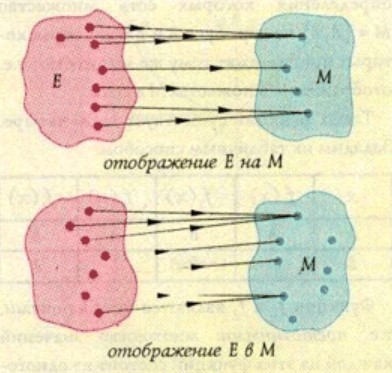
\includegraphics[width = 0.5\textwidth]{ris_1}}

\caption{}
\label{fig:pic_1 }
\end{figure}
М, но не утверждается, что любой элемент
этого множества является значением функции f,
 то говорят, что функция отображает
свою область определения Е в множество М
или что отображение f есть отображение
множества Е в множество М (рис. \ref{fig:pic_1}).

Таким образом, надо строго различать
смысл выражений

{\em «отображение на множество М»,

«отображение в множество М»}

Например, про отображение
$$x \rightarrow |x|$$
можно сказать, что оно является отображе
нием {\bf R в R }, но нельзя сказать, что это отображение {\bf R на R} .

С чисто логической точки зрения наибо
лее простым случаем является случай, когда
область определения функции конечна.
Ясно, что функция, область определения ко
торой состоит из элементов, не может
принимать более п различных значений. Та
ким образом, функции, определенные на
конечных множествах, осуществляют ото
бражения конечных множеств на конечные
множества. Такие отображения являются
одним из предметов изучения важной части
математики - комбинаторики.

{ \bf Пример 4.} Рассмотрим функции, область
Заметьте еще, что каждое отображение можно
назвать и отобрание
но не наоборот.

\end{multicols}











